%% wlkr
\documentclass{article}
\usepackage[hidelinks]{hyperref}
\usepackage{graphicx}
\usepackage{float}
\usepackage{listings}
\usepackage{tikz}
\usepackage{pdfpages}
\usetikzlibrary{positioning}
\usepackage[margin=1in]{geometry}
\usepackage{setspace}
\doublespacing

\lstset{
  basicstyle=\scriptsize, %or \small or \footnotesize etc. 
  commentstyle=\color{red},
  keywordstyle=\color{blue},
  showstringspaces=false,
  breaklines=true,
  aboveskip=1em,
  belowskip=1em
}

\tikzset{%
  every neuron/.style={
    circle,
    draw,
    minimum size=1cm
  },
  neuron missing/.style={
    draw=none, 
    scale=4,
    text height=0.333cm,
    execute at begin node=\color{black}$\vdots$
  },
}

\begin{document}
\begin{center}

\includegraphics[width=6cm]{img/bcit-logo.png} \\
\huge{Bird Density, with Edge ML} \\
\large{by} \\
\large{Ryan Walker and Jin Seo} \\
\vspace*{\fill}
\large{\textbf{Bachelors of Technology in Electronics}} \\
\large{Electrical and Computer Engineering Technology} \\
\large{British Columbia Institute of Technology} \\
\large{December - 2019} \\
\end{center}
\newpage
\begin{center}
\huge{Bird Density, with Edge ML} \\
\large{by} \\

\large{\textbf{Ryan Walker}} \\
\large{Diploma in Robotics and Mechatronics, BCIT, 2011} \\
 
\large{\textbf{Jin Won Seo}} \\
\large{Diploma of Computer Control in ECET, BCIT, 2011} \\
\vfill
\large{\textbf{Bachelors of Technology in Electronics}} \\
\large{ELECTRICAL AND COMPUTER ENGINEERING TECHNOLOGY} \\

\vfill
\large{We accept this report at conforming to the required standard} \\
\large{.............................................................} \\
\large{.............................................................} \\
\large{.............................................................} \\
\large{.............................................................} \\


\vspace*{\fill}
\large{\textbf{Bachelors of Technology in Electronics}} \\
\large{Electrical and Computer Engineering Technology} \\
\large{British Columbia Institute of Technology} \\
\large{December - 2019} \\
\end{center}
\newpage

\tableofcontents
\newpage

\listoffigures
\newpage

\section{Introduction}
Biologists have been aiming to understand bird migration for decades. Various custom hardware has been developed for doing this \cite{BirdTracking}, however is it costly an requires capture and release of the bird. We are proposing the design, construction and deployment of a device that resides in a stationary location. This device is equip with a microphone and microcontroller, and by using machine learning techniques \cite{ML1} \cite{ML2} can detect and speciate various types of birds. In addition the device will also be able to record various types of environmental data for cross-correlation with bird density in post processing. Following the successful deployment we desire to make a bird density heat map of various regions and to undestand how it changes over time.

\section{Machine Learning on the Edge}
\begin{center}
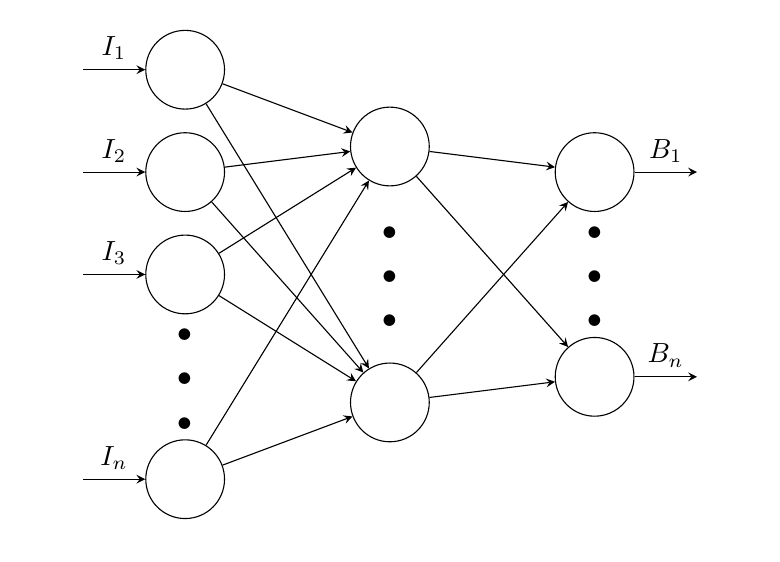
\begin{tikzpicture}[x=1.3cm, y=1.3cm, >=stealth]
\foreach \m/\l [count=\y] in {1,2,3,missing,4}
  \node [every neuron/.try, neuron \m/.try] (input-\m) at (0,2.5-\y) {};

\foreach \m [count=\y] in {1,missing,2}
  \node [every neuron/.try, neuron \m/.try ] (hidden-\m) at (2,2-\y*1.25) {};

\foreach \m [count=\y] in {1,missing,2}
  \node [every neuron/.try, neuron \m/.try ] (output-\m) at (4,1.5-\y) {};

\foreach \l [count=\i] in {1,2,3,n}
  \draw [<-] (input-\i) -- ++(-1,0)
    node [above, midway] {$I_\l$};

\foreach \l [count=\i] in {1,n}
  \draw [->] (output-\i) -- ++(1,0)
    node [above, midway] {$B_\l$};

\foreach \i in {1,...,4}
  \foreach \j in {1,...,2}
    \draw [->] (input-\i) -- (hidden-\j);

\foreach \i in {1,...,2}
  \foreach \j in {1,...,2}
    \draw [->] (hidden-\i) -- (output-\j);

\end{tikzpicture}
\end{center}

Machine learning and AI have been popular topics in the last couple of years, especially the use of neural networks in classification algorithms. A neural network is a collection of artificial neurons which can loosely model the neurons in a biological brain. They are connected is a way that allows data to propagate through them, each neuron connection (edge) has a weight associated with it, this weight either increases or decreases the strength of the signal at a connection. The neurons are arranged in ``layers", the first and last layers are known as the input and output layers respectively, and the middle layers are known at the hidden layers. ``Training" a neural network is the automated process of adjusting the weights on a sample dataset so that the output gives the requred value for a given input. As an example, if were given a problem to classify 1000 pictures into either ``hotdog" or ``not hotdog", where the images were 250 pixels by 250 pixels. You would start by:

\begin{itemize}
\item Manually label a sufficiently large section of the dataset (say 500 pictures)
\item Introduce 62500 input neurons ($250 \cdot 250$)  
\item Introduce 1 output neurons (Hotdog or not hotdog)  
\item Train the network so output says hotdog for all the hotdog pictures, and not hotdog for all the not hotdog pictures
\item When you then feed in puctures it hasn't seen before, it should classify the remaining data correctly
\end{itemize}

The accuracy is given by the ratio of correct classifications to incorrect classifications. It has not been until recently that these applications have moved into edge compute, meaning all the processing is run on the device as apposed to cloud. We propose to design a NN (Neural Network) that can be run on a STM32 microcontroller for classification of various birds. As this is such a rapidly expanding field there are various software implementations developed for embeded applications \cite{CMSIS} \cite{TF}. 

\section{Signal processing}
This project is required to utilize several signal processing techniques. Some of these techniques could be included filters, discrete Fourier transforms, and so on. Filters are necessary to improve the quality of the bird calls and remove unwanted noises. In addition, in order to come up with digitized data from acoustic analog signals, other techniques could be applied such as Discrete wavelet transform or mel-frequency cepstrum. In this case, MATLAB can be used for simulation.

\subsection{Mel Spaced Filter Bank}
Human hearing sensitivity works in a very nonlinear way. For a human, there is a stark difference between a signal that is 50hz and a signal that is 150hz. However is it almost impossible to notice a difference between a a 10khz signal and a 11khz signal. The mel scale has been developed to represent this. It it shown in Equation \ref{mel-eq} and is plotted in Figure \ref{mel}. 

\begin{equation}
M(f) = 1125 \cdot log(1+\frac{f}{700})
\label{mel-eq}
\end{equation}

\begin{figure}[h]
\centering
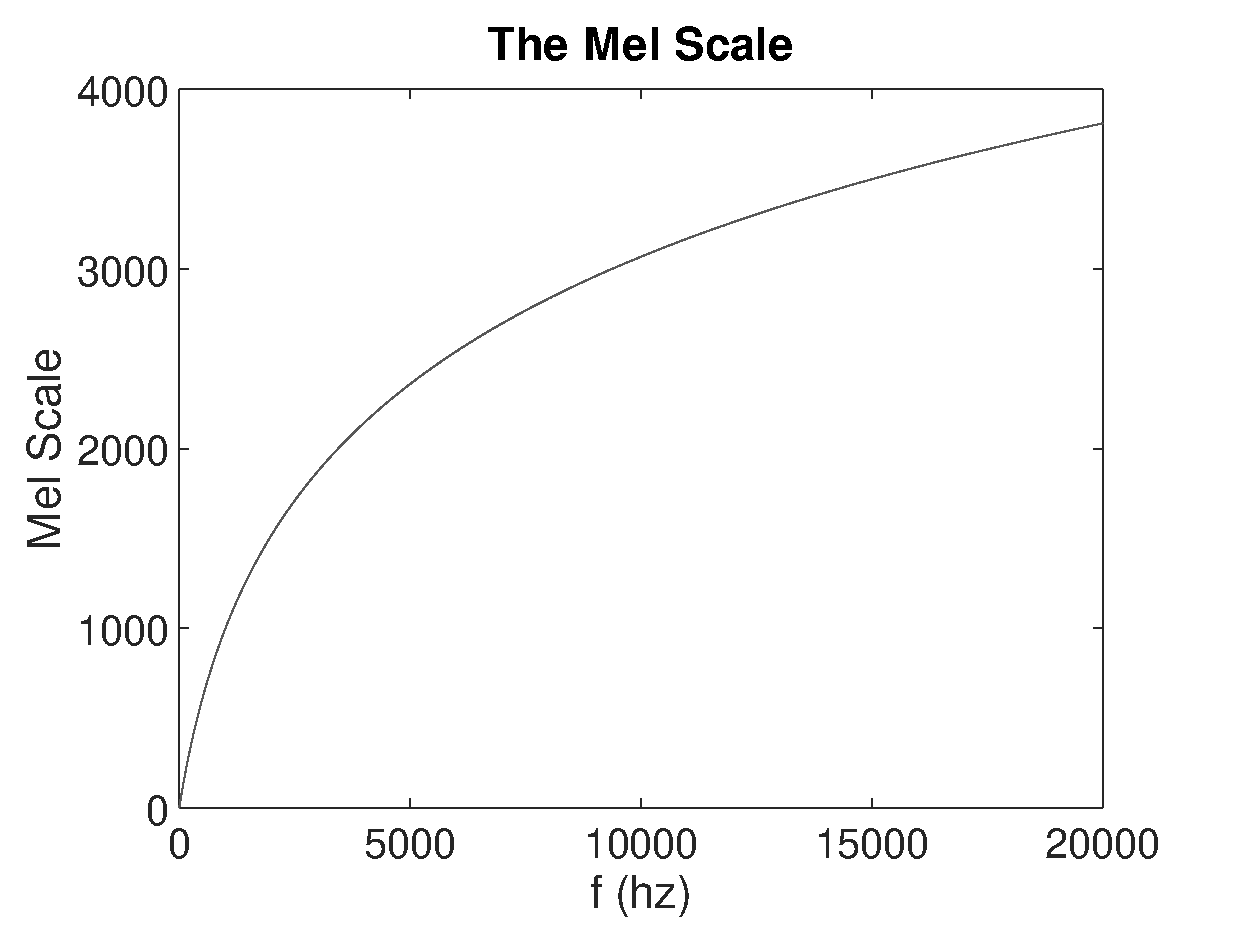
\includegraphics[width=9cm]{mel.eps}
\caption{The Mel Scale}
\label{mel}
\end{figure}

To get more adequate feature extraction we are going to use a mel spaced filter bank. This effectively maximizes the features extracted as a function of the mel scale. The filter array is shown in Figure \ref{FA}. In this example we have implemented ten filters for visulizing purposes, however in practice we are going to implement over twenty.

\begin{figure}[H]
\centering
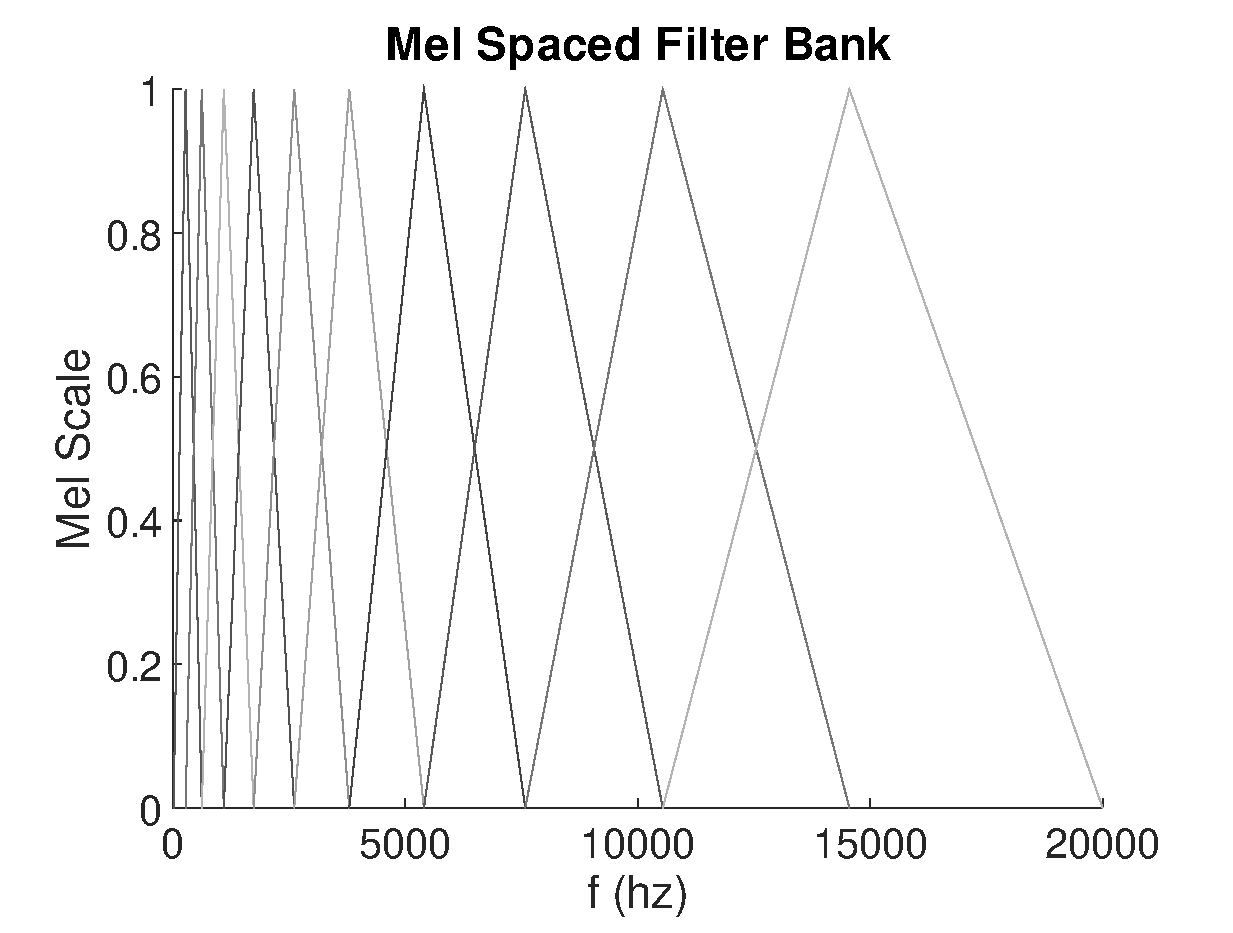
\includegraphics[width=9cm]{FA.eps}
\caption{The Mel Space Frequency Array}
\label{FA}
\end{figure}

\section{Software} In the project we are planning on using Matlab/Simulink for any filter design, C/C++ for embedded code and possibly some python for post processing.

\section{Hardware}
The hardware will need to be battery powered in order to collect data over extended periods of time. We are currently targeting the specifications below.

\begin{center}
\begin{tabular}{ c | c }
Spec             & Metric\\ 
\hline 
Battery Life     & 1 week\\
Compatable Birds & 10    \\
Cost (QTD 100)   & $<\$30$  \\
\end{tabular}
\end{center}

It should be inexpensive so it becomes feasible to deploy many devices and should be completely stand alone. In addition it should have a wiresless uplink/downlink to transmit data to and from a computer.

\subsection{Microcontroller}
In addition to having experience with the STM32 family of microcontrollers, TensorFlow Embedded \cite{TF} has extensive documentation for implementation on the STM32F746 \cite{STM}. This part has 1MB flash, 320k RAM and runs at 216Mhz. TensorFlow embedded is designed to run on 20k of flash, so we will have more than enough space for the NN and application code.

\subsection{Microphone}
The device will contain a microphone that will be used to record ambient noises. A suitable microphone has not yet been selected.

\subsection{Architecture}
\begin{itemize}
\item{\textbf{MCU:} STM32F746.}
\item{\textbf{SD card:} For recording data.}
\item{\textbf{18650 Cell:} 2x 18654 Li-ion cells for power.}
\item{\textbf{Microphone:} Microphone for recording sound.}
\item{\textbf{Temperature Sensor:} Temperature sensor for recording ambient temperature.}
\end{itemize}

\section{Data Harvesting and Conditioning}
In order to train the neural net, we require a great deal of data. This was gatherd from a website where bird listeners post sounds of birds \cite{Bird}. To this day we have gathered and labeled 589 crow samples, of which roughly half are not crows and 691 sanpiper samples to which roughly half are not sanpipers. We did this using the workflow outlined below.

\subsection{Harvesting}
The script below harvest the data from a given bird.
\lstinputlisting[language=bash]{../NN/data/fetch.sh}

\subsection{Labeling}
The labeling process was done manually, it was done with the script below essentually this script will hunt through a file and find sound files, then it will chunk off a 1s piece and play it, if the user presses 'y' then it will save the file down as ``n\_crow" if the user pressed 'n' then it will save the file down a ``n\_Notcrow", where n is an incremented integer.
\lstinputlisting[language=python]{../NN/data/splice.py}

\subsection{Conditioning}
Our neural network is deigned to accepts frequency data, not sound data. So there is some conditioning required beforehand. This script opens up the output files from the last script and preforms a FFT. It then reduces the number of bins to something more manageable, right now we are using 128 input neurons, so there are 128 fft bins. It then saves all this to a single json file. 
\lstinputlisting[language=python]{../NN/data/fft.py}

\section{The Neural Network}
\subsection{Background and Exsisting work}
The idea of Artificial Neural Networks comes from the structure and functions of a human brain. Neurons in human brain that process and transmit information between themselves.
\begin{figure}[H]
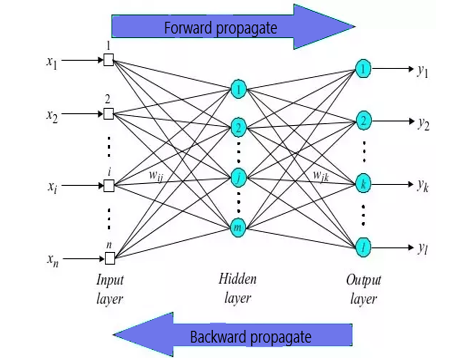
\includegraphics[scale=0.65]{img/NN_general.png}
\centering
\caption{Forward\&Backward Neural Network}
\end{figure}

\subsubsection{Perceptron}
Perceptron that functions as a step function was used to model of decision-making.Thus, if perceptron is over a certain threshold, it outputs 1 otherwise 0.
Perceptrons act as a linear decision; however, many reality functions are NOT linear.
\begin{figure}[H]
  \centering
  \begin{minipage}[b]{0.3\textwidth}
    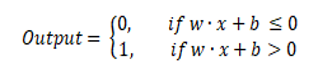
\includegraphics[width=\textwidth]{img/percept.png}
    \caption{equation of perceptron.}
  \end{minipage}
  \hfill
  \begin{minipage}[b]{0.5\textwidth}
    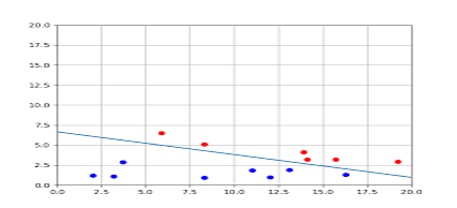
\includegraphics[width=\textwidth]{img/percept2.png}
    \caption{linearity of perceptron.\protect\cite{Percept}}
  \end{minipage}
\end{figure}

\subsubsection{Sigmoid}
Sigmoid neuron has weights for each input w1,w2,\dots , and overall bias b. 
It’s $\sigma{(w \cdot x+b)}$ which is called the sigmoid function
So, the sigmoid can be expressed as:

$\sigma{(z)} =\frac{1}{1+\exp(-z)} \dots (3)$ 
, $a =\frac{1}{1+\sum_{-j}\exp(-w_jx_j-b)} \dots  (4)\cite{NN}$

\begin{figure}[H]
\centering
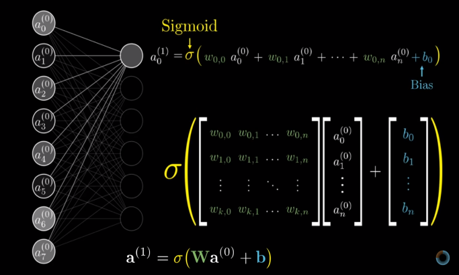
\includegraphics[scale=0.75]{img/sig_eqn.png}
\caption{Activated output neurons with sigmoid.\protect\cite{DL}}
\label{sig}
\end{figure}

The Neural network could have multiple layers, so in that case, input of the sigmoid function could be the output of a neuron from previous layer. As shown in figure \ref{sig} Different combinations of the activated output neurons fire different neurons in the next layer.

\subsubsection{Learning with Gradient descent}

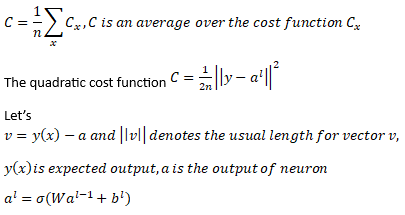
\includegraphics[scale=0.8]{img/gradient.png}

\begin{figure}[H]
  \centering
  \begin{minipage}[b]{0.4\textwidth}
    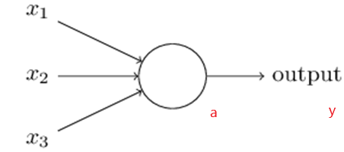
\includegraphics[width=\textwidth]{img/gradient1.png}
    \caption{Cost function.}
    \label{cost}
  \end{minipage}
  \hfill
  \begin{minipage}[b]{0.5\textwidth}
    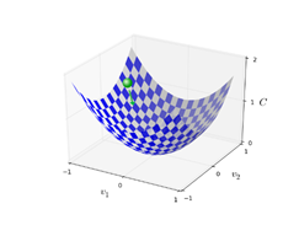
\includegraphics[width=\textwidth]{img/gradient2.png}
    \caption{Gradient descent}
  \end{minipage}
\end{figure}
As shown in the figure \ref{cost},the cost is differences between the expected output and the actual outcome from a neuron . Our goal is to find a weights and biases that minimize the cost. This is known as gradient descent.Gradient ,in mathematics, means the direction of steepest increase. In other words, find a local minimum by training NN.
$\\a^l =\sigma{(wa^{l-1}+b)} \dots (22)\cite{NN} ,\\
z^l_k =\sum_{j}-w^l_{kj}a^{l-1}+b^l_k \dots  (23)\cite{NN}\\$
Where $a^l$ is the vector of activations of neuron in the next layer, $a^{l-1}$ is the vector of activations of previous layer of neurons. z is weighted input.

\begin{figure}[H]
\centering
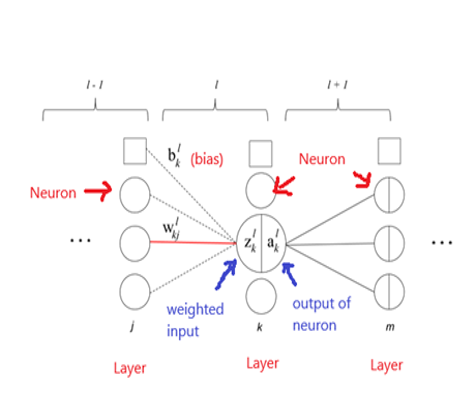
\includegraphics[scale=0.75]{img/forward.png}
\caption{Forward propagatoin.}
\label{forward}
\end{figure} 
Unfortunately, when the number of training inputs is very large this can take a long time and learning thus occurs slowly. So, stochastic gradient descent can be used to speed up learning. The idea is to estimate the gradient C by computing $C_x$ for a small sample of randomly chosen training inputs\protect\cite{NN}Ch2.

\subsubsection{Backward Propagation}

\begin{figure}[H]
  \centering
  \begin{minipage}[b]{0.8\textwidth}
    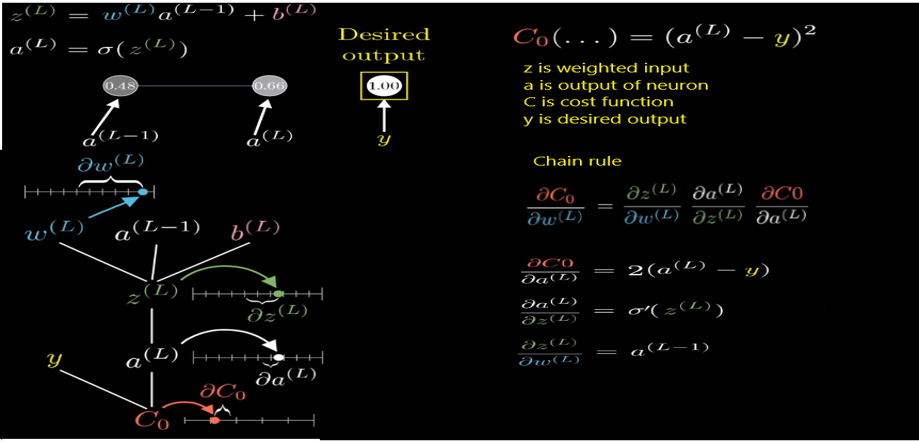
\includegraphics[width=\textwidth]{img/backprop.png}
    \caption{Backward propagation.\protect\cite{DL}}
    \label{back}
  \end{minipage}
  \hfill
  \begin{minipage}[b]{0.3\textwidth}
    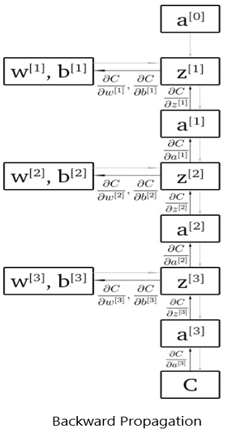
\includegraphics[width=\textwidth]{img/backprop2.png}
    \caption{Diagram of Backward propagation.\protect\cite{BK}}
    \label{back2}
  \end{minipage}
\end{figure}

The forward propagation doesn’t give us the best result. As mentioned before, we want to find a set of weights and biases to minimize the cost by computing gradient ,and this algorithm is known as the backward propagation.
As shown the figures \ref{back} and \ref{back2}, partial derivative and chain rule drive the network backward.
Small changes of weights change the cost; therefore, the chain rule can be applied to explain this phenomenon.
$\frac{\partial C_0}{\partial w^L} = \frac{\partial z^L}{\partial w^L}\frac{\partial a^L}{\partial w^L}\frac{\partial C_0}{\partial a^L}\dots (7.1)\\$
As we take a derivative of each terms.
$\\ \frac{\partial z^L}{\partial w^L}=a^{L-1} \dots (7.2)
\\ \frac{\partial a^L}{\partial z^L}=\sigma^{'}(z^L) \dots (7.3)
\\ \frac{\partial C_0}{\partial w^L} = 2(a^L - y) \dots (7.4)$
\\As you see the term $,\frac{\partial z^L}{\partial w^L}=a^{L-1},$ partial derivative gives us the activated output neuron in the previous layer. This doesn't explain whole equations of backward propagation, but it gives us an idea how the backward propagation works.

\subsubsection{Cross-entropy Cost function}
As shown in the sigmoid \ref{sig}, if the neuron's output get close to 1, the curve gets flat, so $\sigma^{'}(z)$ get very small (slow down).
Cross-entropy avoids the problem of slowdown by vanishing the term $\sigma^{'}(z)$

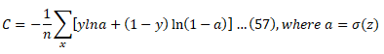
\includegraphics[scale=0.8]{img/cross.png}, 
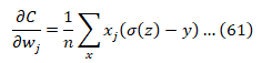
\includegraphics[scale=0.6]{img/cross1.png}

the term $\sigma^{'}(z)$ disappears in the equation (61) after derivative of the cost with respect to weight.

\subsubsection{Training,Validation,and Early stopping}
In training process, separate training and validating data so as to evaluate NN model. In a training process, we define the number of epochs that iterates forward and backward propagation. Perhaps people think of increasing the number of epochs leads us to achieve the better result. However, there is a problem called over fitting. Over fitting (Over training) is a situation where the cost of training data decreases but the accuracy of validating data gets saturated.
Once the classification accuracy on the validation data has saturated, we stop training (Early stopping).
\begin{figure}[H]
  \centering
  \begin{minipage}[b]{0.4\textwidth}
    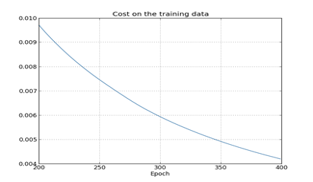
\includegraphics[width=\textwidth]{img/over.png}
    \caption{Decreasement of cost as epochs increases in training data.\protect\cite{NN}}
    \label{over}
  \end{minipage}
  \hfill
  \begin{minipage}[b]{0.4\textwidth}
    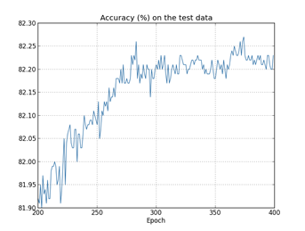
\includegraphics[width=\textwidth]{img/over1.png}
    \caption{Saturation of accuracy in validating data.\protect\cite{NN}}
    \label{over1}
  \end{minipage}
\end{figure}

To avoid overfitting. Then save the hyper-parameters (\# of epochs, learning rate,...). The learning rate is how fast the network learns; however, the network learning fast could cause over-shooting in the gradient descent.
Repeating training by modifying the NN model and parameters until getting good accuracy.

\subsubsection{Other NN model - Convolutional NN}

Another type of NN called Convolutional NN. $a^l=\sigma{(a^{l-1}*w+b)}$and $\ast$ is called a convolution operation.
\\Activation of CNN = $\sigma{(b+\sum_{l=0}^{n}\sum_{m=0}^{n}-w_{l,m}a_{j+l,k+l})} \dots  (125)\cite{NN}$
\begin{figure}[H]
  \centering
  \begin{minipage}[b]{0.6\textwidth}
    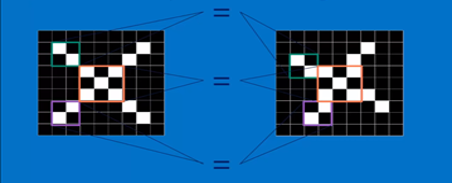
\includegraphics[width=\textwidth]{img/convol.png}
    \caption{Break down maps and features in CNN.\protect\cite{CON}}
    \label{over}
  \end{minipage}
  \hfill
  \begin{minipage}[b]{0.6\textwidth}
    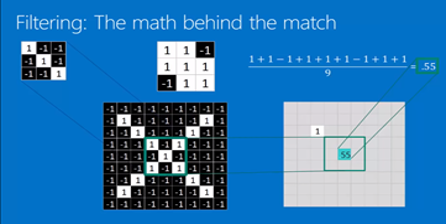
\includegraphics[width=\textwidth]{img/convol1.png}
    \caption{Parameters reducing by CNN.\protect\cite{CON}}
    \label{over1}
  \end{minipage}
\end{figure}

As you see in the figure \ref{over1}, the outcome of filtering is compressed by the filtering steps. In other words each element doesn’t have own weights and biases, they share weights and biases!.

Filtering steps {\protect\cite{CON}}:
\begin{itemize}
\item Line up the feature and map
\item Multiply each element of map by corresponding feature element
\item Add them up
\item Divide by the total number of elements in the feature
\end{itemize}
A big advantage of sharing weights and biases is that it greatly reduces the number of parameters involved in a convolutional network.
What is good about reducing the number of parameters? First,it speeds up the computation. Second,it gives us better accuracy.An example of using image pixels has been used to explain CNN.
What’s about our case? Our input getting into the NN is MFCC(Mel Frequency Cepstral Coefficients). As we visualize the data of MFCC, it does not look quite different from the image data!.A spectrogram is a visual representation of the spectrum of frequencies of a signal as it varies with time. 

\begin{figure}[H]
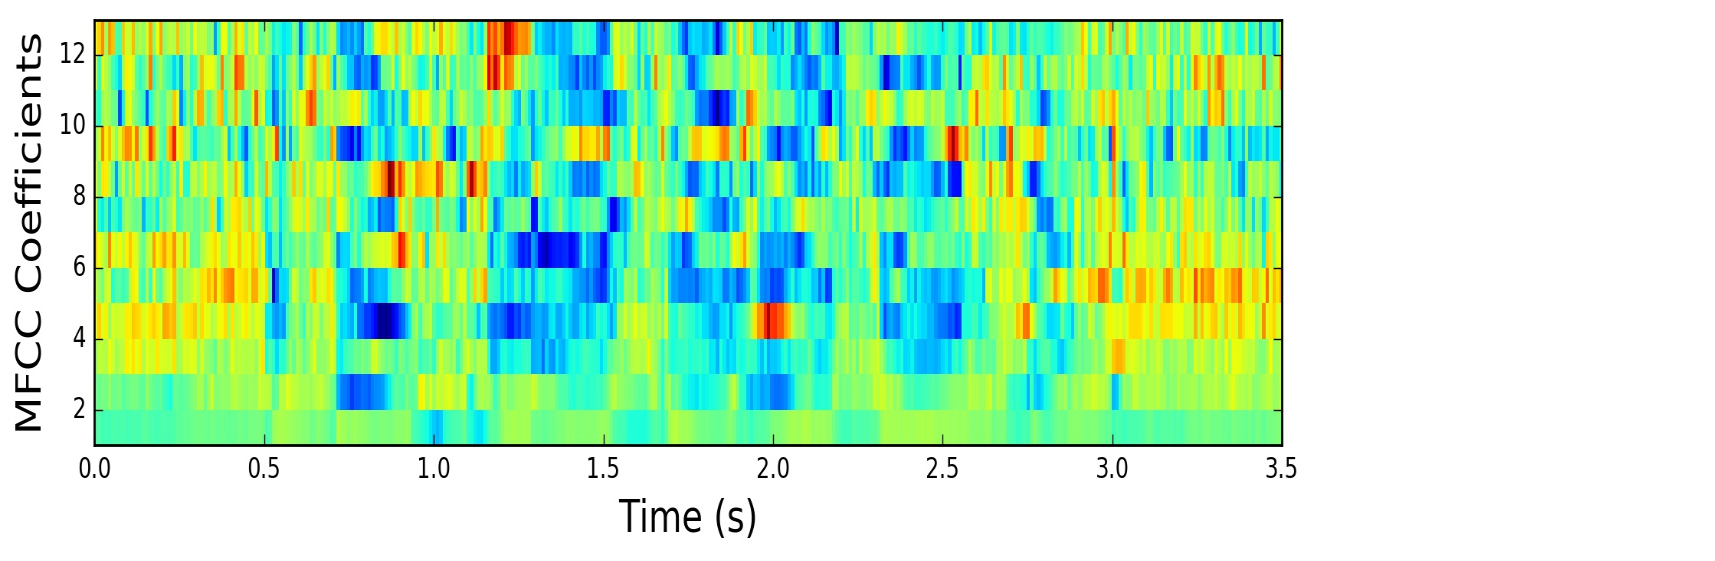
\includegraphics[scale=0.25]{img/MFCC.png}
\caption{MFCC \protect\cite{AU}}
\label{mfcc}
\end{figure}

\subsubsection{Max-pooling}
In max pooling, a pooling unit simply outputs the maximum activation in the N×N input region.
Pooling steps {\protect\cite{CON}}:
\begin{itemize}
\item Pick window size( 2 or 3)
\item Pick stride size (usually 2)
\item Walk the window across the filtered outputs (CNN)
\item From each window, take the maximum value
\end{itemize}

\begin{figure}[H]
  \centering
  \begin{minipage}[b]{0.6\textwidth}
    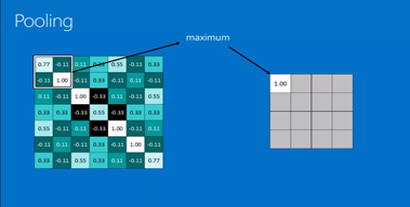
\includegraphics[width=\textwidth]{img/max.png}
    \caption{Max-pooling.\protect\cite{CON}}
    \label{max}
  \end{minipage}
  \hfill
  \begin{minipage}[b]{0.6\textwidth}
    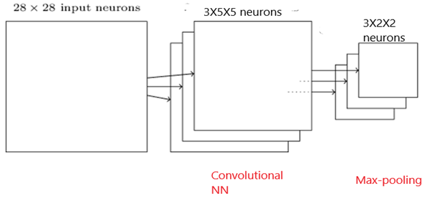
\includegraphics[width=\textwidth]{img/max1.png}
    \caption{Model of CNN and Max-pooling.\protect\cite{DL}}
    \label{max1}
  \end{minipage}
\end{figure}

\hfill \break A big benefit is that this helps reduce the number of parameters needed in later layers as shown in the figure \ref{max},

\subsubsection{Other activation function - Rectified Linear Units (ReLU)}
The concept and example of Neural Network that we have dealt with so far use the one activation function which is the sigmoid. There are different type of activation functions and one of those is Rectified Linear Units.
\begin{figure}[H]
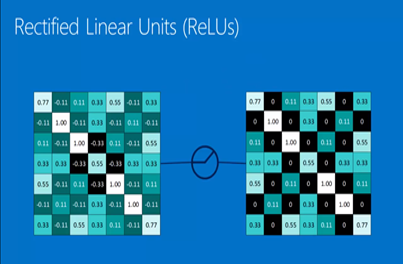
\includegraphics[scale=0.8]{img/relu.png}
\caption{ReLu \protect\cite{CON}}
\label{rele}
\end{figure}
\hfill \break ReLu nomalizes the output of NN by tweaking each of values just a bit ex) change every negative values to zero \cite{DL}.
People found that networks based on rectified linear units consistently outperformed than networks based on sigmoid activation functions.However,it has shown that ReLu is empirically better( Not mathematically proved).

\subsection{Put all together}

\begin{figure}[H]
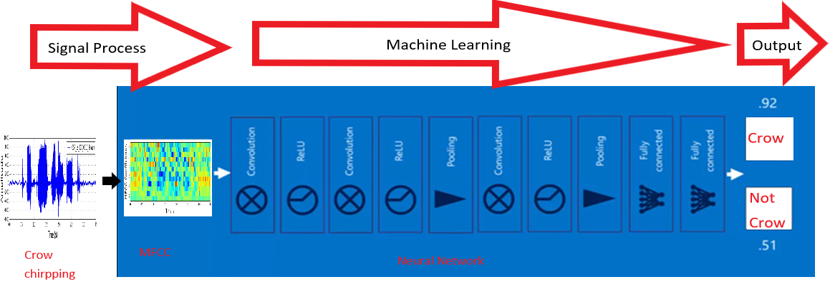
\includegraphics[scale=0.7]{img/all.png}
\caption{Model of Birdear}
\label{mod}
\end{figure}
As shown in the figure \ref{mod}, signals of bird chirpping go into our the signal process. It ends up composing the MFCC, which is the input of NN. In the end, the NN distingusih what kind of bird is.

\subsection{Software Appication(PC) and Experiments}
We chose Tensorflow for out neural network design because one you train up a model, you have the ability to convert it to a ``tflite" model which can be run on a microcontroller using tensorflow lite. We then built the model structure and trained the model. Our current model is shown in Figure \ref{model}, it has 128 input neurons on the input layer (for our 128 fft bins) 128 neurons on the one hidden layer and 1 neuron on the out (either crow or not crow). The script starts by randomly splitting our dataset into the training and validation set, where the training set it used for the training while the validation set is used for validation after the training is complete, that is to say the network has no knowledge of the validation set when adjusting the weights. After this process our network got \textbf{93\% accuracy on the validation set}

\section{Hardware}
The first revision of the hardware is finished and we have connected to the microcontroller, we have blinked on of the LEDs but have not implemented any sampling or the neural network. The physical hardware is shown in Figure \ref{hardware} while the schematic is shown in Figure \ref{sch1} and \ref{sch2}. We got a PCB manufactued overseas ans placed all the SMD components onto it.
 
\begin{figure}[H]
\centering
\includegraphics[scale=0.07]{img/E04A0175.JPG}
\caption{Hardware}
\label{hardware}
\end{figure}

\begin{figure}[H]
\centering
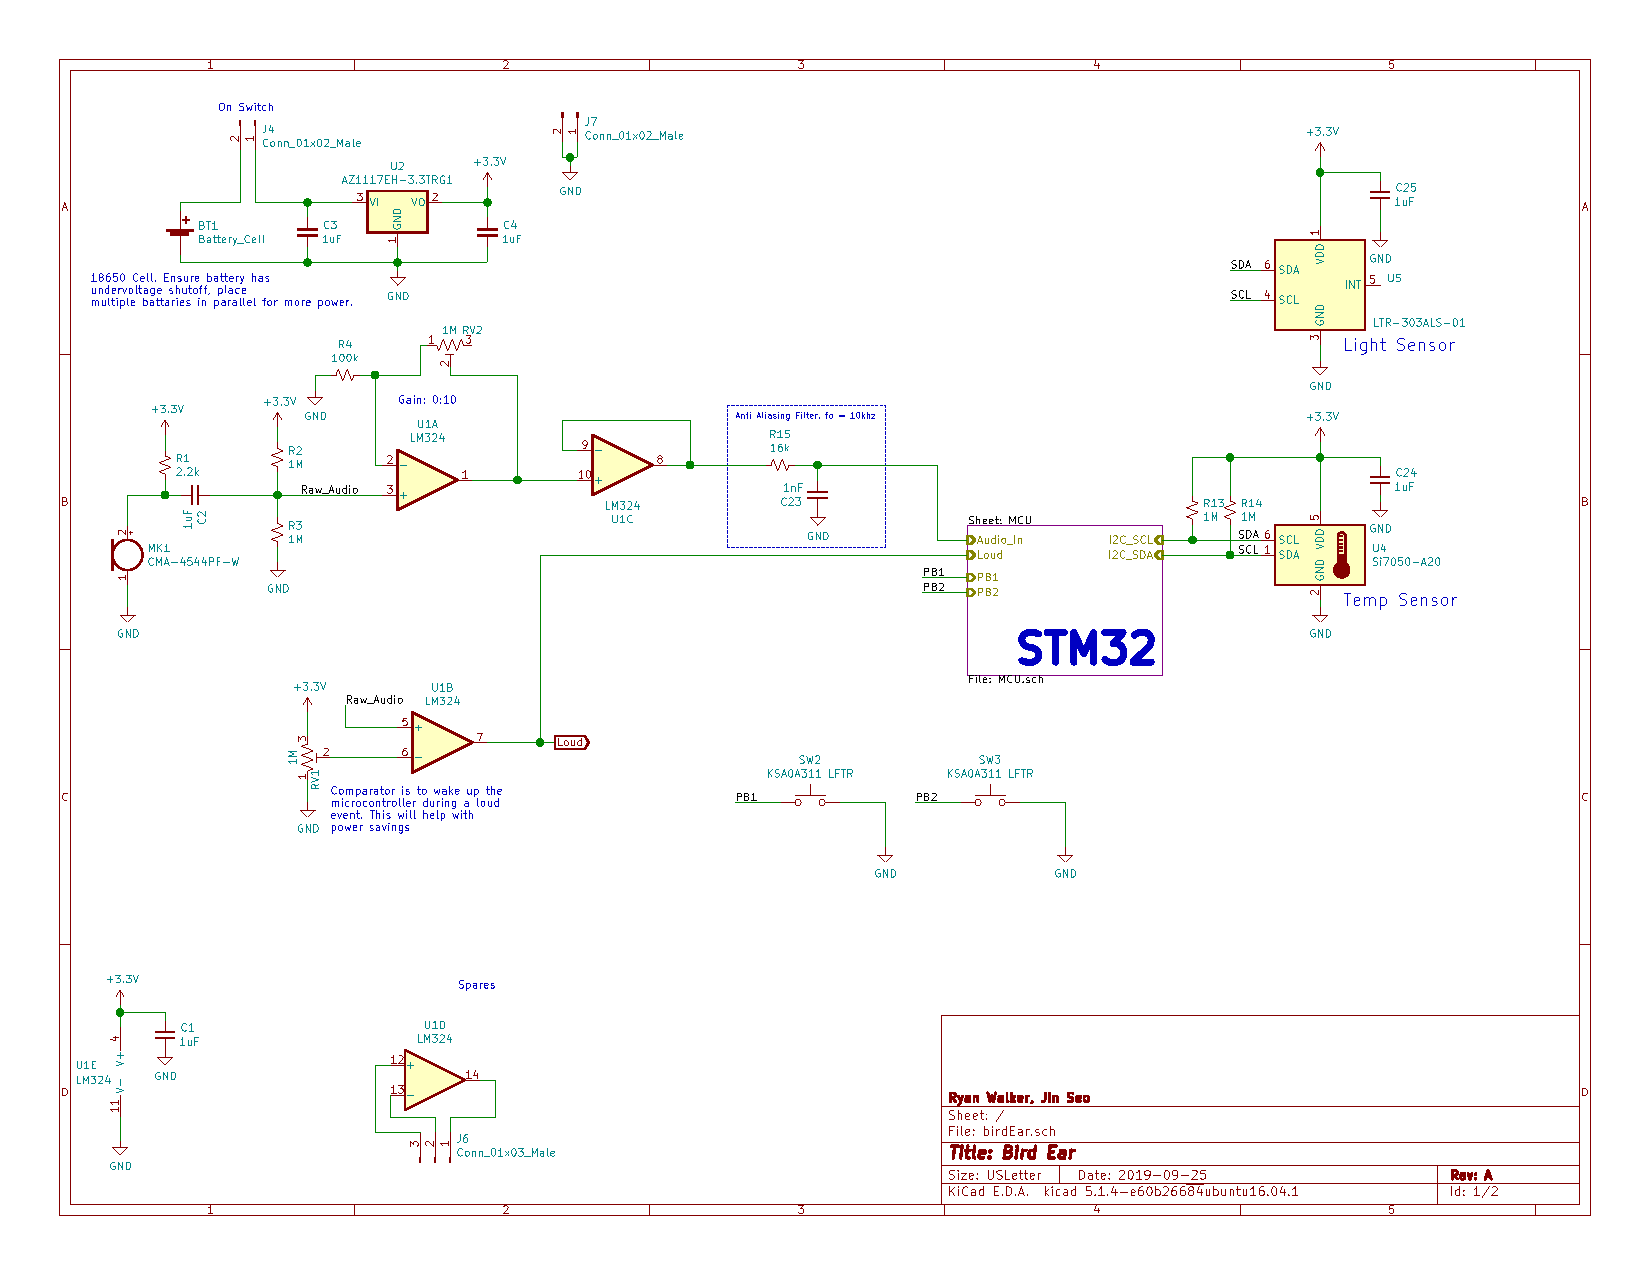
\includegraphics[scale=0.7, angle=90, page=1]{../birdEar/plot/birdEar.pdf}
\caption{Schematic - page 1}
\label{sch1}
\end{figure}

\begin{figure}[H]
\centering
\includegraphics[scale=0.7, angle=90, page=2]{../birdEar/plot/birdEar.pdf}
\caption{Schematic - page 2}
\label{sch2}
\end{figure}

\section{Conclusion}
As mentioned in the section "Data Harvesting and Conditioning",
we have gathered and labeled 589 crow samples, of which roughly half are not crows and 691 sanpiper samples to which roughly half are not sanpipers. Those samples are stored as WAV formats so that the modules of signal process can extract MFCC at the end of the process. Since MCU has a limited resources, it is necessary to compress digital data as much as possible. However, just compressing data into MCU is not our goal. The idea is how much signal data could be compressed without lossing discrete digital data in low frequency range. In other words, the compressed data still should represent the features of the original signal.\\
Sound of birds' chirpping keeps changing abrumptly in a short time; therefore, it may not make so much sense to take FFT(Fast Fourier Transform) in the whole signal. In this case, STFT (Short time Fourier Transform) could be better solution. In addition, applying DCT(Discrete Cosine Transform) could help to decompose the overlapped signals from the STFT and compress data. The reason to come up with MFCC(Mel Frequency Cepstral Coefficients) is that first, it allows to shrink down the size of inputs. Second, it filters out signals in high frequency range, and focuses on the human perceivable hearing range (low frequency range). Our goal is not making some high quality audio sounds; rather, we are processing the signals such that NN can be discriminative enough between the birds' chirpping.Perhaps, the testing result of NN,around 93\%, still looks promissing with our testing samples; however, in order to solidify the model of NN, more diverse data could be required. The more varioud data we have, the better accuracy the NN performs. But, getting more data results in expensive cost since it takes a time and efforts.\\
Unlike the other typical embedded system projects that are directly designed and implemented on MCU. Our project requires pre-steps before attacking MCU, which is to verify the model in the environments of PC. Although PCs and embedded systems are quite different in a matter of archetecture and resources, it seems to be inevitable to work on PC first. The reasons behind is that first, Machine Learing is still a new area for the embedded systems. Another reason is lots of resources of NN work based on PC, so without getting through the test based on PC, it is hard to estimate that the model of NN works on the embedded systems.\\
From this project, we have been exposed ourselves to a new rising technical area, Neural Network, to see if it is possible to apply this to the embedded systems. Our answer for this is of course it is possible, and there seems to be area where electrical and electronics engineering could adapt the new rising technique such as signal process, power system, tele-communication, and so on. Moreover, we have learned techniques of the signal process that handle analogue to digital signals demanding compressing data for the embedded systems. 
\newpage

\section{Next Steps}
The next steps of the project are...

\begin{itemize}
\item Implement mel-spaced frequency array.
\item Increase the number output neurons to 2, so we can classify between crows and sandpipers. 
\item Add another three types of birds to the dataset.
\item Research "VGG like feature extraction".
\item Implement microcontroller firmware for audio sampling.
\item Implement neural network on the microcontroller.
\item Deploy the device in the field.
\end{itemize}

\begin{thebibliography}{1}

\bibitem{BirdTracking}
Bird Tracking Hardware.
\url{https://atstrack.com/animal-class/avian.aspx} [Accessed June 22, 2019]

\bibitem{ML1}
Stowell, Wood, Pamuła, Stylianou4, Glotin "Automatic acoustic detection of birds through deep learning: the first Bird Audio Detection challenge"
\url{https://arxiv.org/pdf/1807.05812.pdf}

\bibitem{ML2}
Ilyas Potamitis, "Deep learning for detection of bird vocalisations"
\url{https://arxiv.org/pdf/1609.08408.pdf}

\bibitem{CMSIS}
CMSIS NN Software Library
https://www.keil.com/pack/doc/CMSIS/NN/html/index.html

\bibitem{TF}
TensorFlow Lite for Microcontrollers
https://www.tensorflow.org/lite/microcontrollers/overview

\bibitem{STM}
ARM® Cortex®-M7 STM32F7 Microcontroller IC 32-Bit 216MHz 1MB (1M x 8) FLASH 100-LQFP (14x14)
https://www.digikey.ca/product-detail/en/stmicroelectronics/STM32F746VGT6/497-15819-ND/5287178

\bibitem{Bird}
xeno-canto is a website dedicated to sharing bird sounds from all over the world.
https://www.xeno-canto.org/

\bibitem{BirdCallIdentifier}
Bird Call Identifier.
\url{https://web.wpi.edu/Pubs/E-project/Available/E-project-042910-001603/unrestricted/Bird_Call_Identification_MQP_2010.pdf} [Accessed April 29, 2010]

\bibitem{Percept}
Calculate the Decision Boundary of a Single Perceptron,
Tomas Countz,
\url{https://medium.com/@thomascountz/calculate-the-decision-boundary-of-a-single-perceptron-visualizing-linear-separability-c4d77099ef38}, Apri 2018

\bibitem{NN}
Neural Networks and Deep Learning,
Michael Nielsen,
\url{http://neuralnetworksanddeeplearning.com/index.html} [Accessed Determination Press, June, 2019]

\bibitem{DL}
Deep learning,
\url{https://www.youtube.com/watch?v=aircAruvnKk&list=PLZHQObOWTQDNU6R1_67000Dx_ZCJB-3pi&index=1},
2017

\bibitem{BK}
A beginner’s guide to deriving and implementing backpropagation,
Pranav Budhwant,
\url{https://medium.com/binaryandmore/beginners-guide-to-deriving-and-implementing-backpropagation-e3c1a5a1e536}

\bibitem{CON}
How Convolutional Neural Networks work,
Brandon Rohrer,
\url{https://www.youtube.com/watch?v=FmpDIaiMIeA&t=243s},
2016

\bibitem{AU}
Speech Processing for Machine Learning: Filter banks, Mel-Frequency Cepstral Coefficients (MFCCs) and What's In-Between,
Haytham Fayek,
\url{https://haythamfayek.com/2016/04/21/speech-processing-for-machine-learning.html},
April, 2016

\bibitem{MF}
Mel Frequency Cepstral Coefficient (MFCC) tutorial,
James Lyons,
\url{http://practicalcryptography.com/miscellaneous/machine-learning/guide-mel-frequency-cepstral-coefficients-mfccs/}

\end{thebibliography}
\newpage

\appendix
\section{Appendix A}
\subsection{Testing NN codes(Python)}

Following codes represent NN model that has a couple of CNN and a Max-pooling:
\lstinputlisting[language=python]{../NN/audio/src/train.py}
\hfill \break
Another simple NN:
\lstinputlisting[language=python]{../NN/audio/src/main.py}

\begin{figure}[H]
\centering
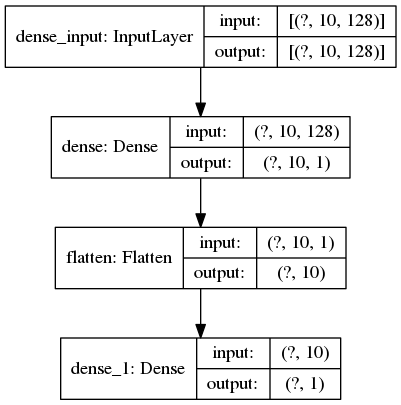
\includegraphics[scale=0.3]{../NN/audio/src/model.png}
\caption{Current Model}
\label{model}
\end{figure}
\newpage
\subsection{Testing Signal Process codes(Python)}
Read .wav that recorded bird chirpping, then feed it into the signal process that outputs MFCC(Mel Frequency Cepstral Coefficients)

\lstinputlisting[language=python]{../NN/data/SignalProcess/stft_mel.py}

\section{Appendix B}
\subsection{List of abbreviations and acronyms}

STFT = Short Time Fourier Transform\\
FFT = Fast Fourier Transform\\
DCT = Discrete Cosine Transform\\
MFCC = Mel Frequency Cepstral Coefficients\\
MCU = Micro Controller\\
PC = Personal Computer\\

\end{document}
